\chapter{Работа №3. Знакомство с сенсорной панелью. Работа с прерываниями}

Цель работы: 
\begin{itemize}
\item Знакомство с существующими технологиями емкостных сенсорных панелей.
\item Настройка и использование стандартной библиотеки по работе с сенсорной панелью.
\item Изучение принципов работы с прерываниями.
\end{itemize}

\section{Описание принципов работы сенсорной панели}
На отладочной плате STM32L-Discovery установлена сенсорная панель, выполненная по емкостной технологии. Существует несколько технологий емкостных сенсорных датчиков

\textit{Измерение времени заряда/разряда RC-цепи} (RC acquisition principle) --- при касании в чувствительной зоне кнопки (чаще всего касание одного из электродов) изменяется емкость, соответственно изменяется постоянная времени цепи, изменение которой регистрируется контролирующей схемой. 
	
	\textit{Опрос датчика путем переноса заряда} (Charge transfer acquisition principle) --- опрос кнопки путем измерения времени заряда измерительного конденсатора разрядом конденсатора, образованного сенсорной кнопкой. В этом случае конденсатор сенсорной кнопки периодически заряжается, а его разряд происходит на другой конденсатор (измерительный, sampling capacitor), и замеряется время его заряда до определенного \textit{порогового напряжения (threshold voltage}). При касании кнопки ее емкость увеличивается (накапливается больший заряд), и заряд измерительного конденсатора происходит за меньшее время.   
	
	\textit{Технология поверхностной емкости }(Surface capacitance). Емкость кнопки изменяется при приближении пальца близко к ее поверхности за счет дополнительной емкости: 
\begin{itemize}
\item До земли через тело человека;
\item Емкости между человеческой рукой и устройством;
\item Емкости между телом человека и печатной платой устройства (наподобие антенны).
\end{itemize}
\begin{figure}[H]
\begin{center}
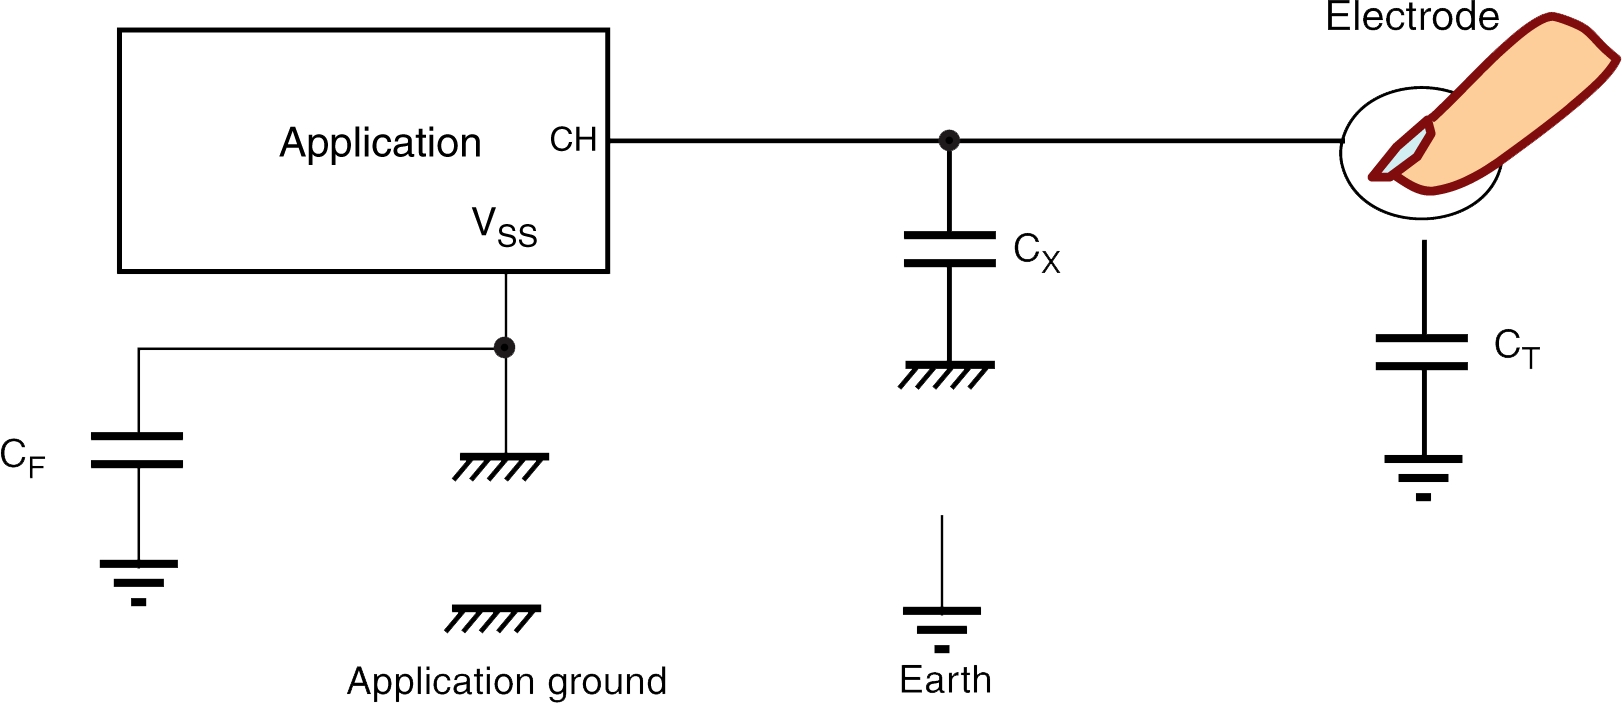
\includegraphics[scale=0.25]{Image/55.jpg} 
\end{center}
\caption{Принцип поверхностной емкости}
\end{figure}

\textit {Cx} --- паразитная емкость электрода.
 
\textit {Cf} --- обратная связь между землей и приложением.

\textit {Ct} --- емкость образованная касанием пальца.

\textit{Проекционная емкость (Projected capacitance)}. При прикосновении изменяется диэлектрическая проницаемость, соответственно изменяется общая емкость.

\section{Опрос датчика путем переноса заряда}

Данный метод является простым и наиболее удобным способом измерения емкости. Суть технологии заключается в том, что все GPIO, подключенные к сенсорной панели (кнопке) объединены в группы по 2 -- 4 порта в каждой. В каждой группе один GPIO выделен для \textit{измерительного конденсатора} (sampling capacitor). Остальные GPIO выделены для электродов и называются \textit{каналами} (channels).

\begin{figure}[H]
\begin{center}
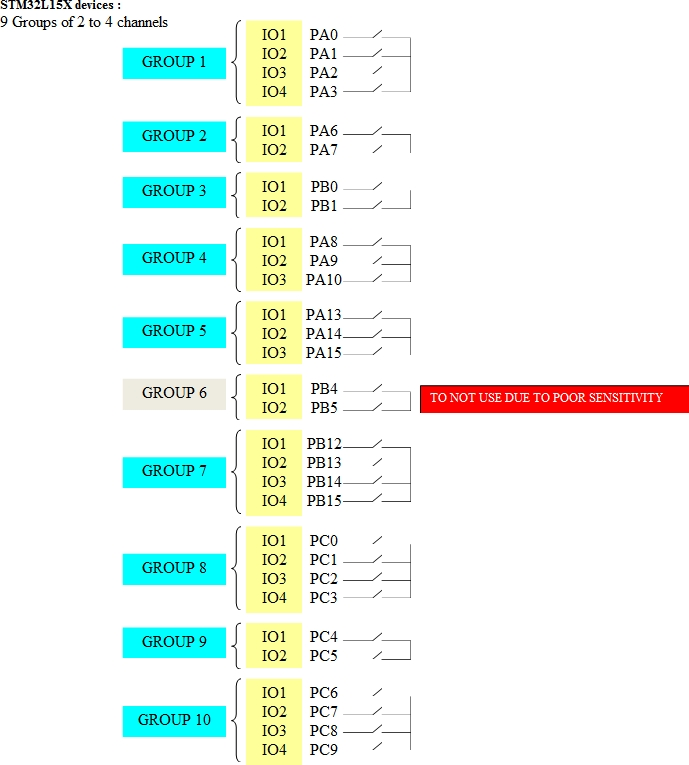
\includegraphics[scale=0.5]{Image/56.jpg} 
\end{center}
\caption{Объединение портов в группы}\label{PortInGroup}
\end{figure}

Принцип переноса заряда состоит в накоплении заряда на конденсаторе \textit{Cx} и его разряде через измерительный конденсатор \textit{Cs}. Разряд повторяется до тех пор, пока напряжение на измерительном конденсаторе \textit{Cs} не достигнет определенного порогового уровня (threshold voltage). В таблице \ref{PerenosZaryada} приведен пример использования технологии опроса датчика путем переноса заряда для первого канала (G1\_IO1), подключенного к кнопке 1. Состояния с 3 по 7 повторяются до тех пор, пока напряжение на измерительном конденсаторе не достигнет порогового значения.


\begin{figure}[H]
\begin{center}
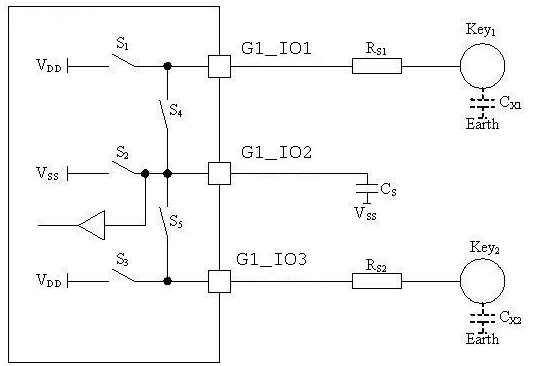
\includegraphics[scale=0.5]{Image/57.jpg} 
\end{center}
\caption{Схема подключения кнопок}
\end{figure}

\begin{figure}[H]
\begin{center}
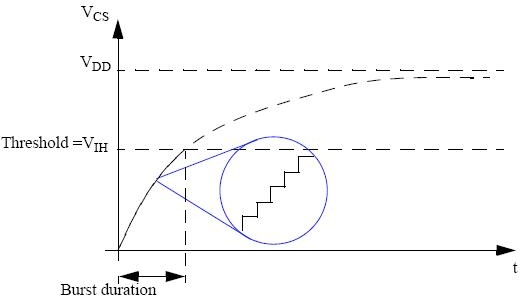
\includegraphics[scale=0.7]{Image/58.jpg} 
\end{center}
\caption{Рост напряжения на измерительном конденсаторе \textit{Cs}}
\end{figure}



\begin{table}[H]
\caption{Опроса датчика путем переноса заряда. Принцип работы}\label{PerenosZaryada}
\begin{center}
\begin{tabular}{|c|>{\centering}m{2cm}|c|>{\centering}m{2cm}|c|c|>{\centering\arraybackslash}m{3cm}|}
\hline
Состояние & Ключ S1 & Ключ S2 & Ключ S3 & Ключ S4 & Ключ S5 & Описание\\
\hline
1 & Открыт & Закрыт & Открыт & Закрыт & Закрыт & Конденсаторы \textit{Cx1, Cx2, Cs} разряжены\\
\hline
2 & Открыт & Открыт & Открыт & Открыт & Открыт & Время простоя (Dead time)\\
\hline
3 & Закрыт & Открыт & Открыт & Открыт & Открыт & Заряд конденсатора \textit{Cx1}\\
\hline

4 & Открыт & Открыт & Открыт & Открыт & Открыт & Время простоя (Dead time)\\
\hline
5 & Открыт & Открыт & Открыт & Закрыт & Открыт & Разряд через конденсатор \textit{Cs}\\
\hline
6 & Открыт & Открыт & Открыт & Открыт & Открыт & Время простоя (Dead time)\\
\hline
7 &Открыт & Открыт & Открыт & Открыт & Открыт & Измерение напряжения на конденсаторе \textit{Cs}\\
\hline
\end{tabular}
\end{center}
\end{table}

%%%%%%%%%%%%%%%%%%%%%%%%%%%%%%%%%%%%%%%%%%%%%%%%%%%%%%%%%%%%%%%%%%%%%%%%%%%%%%%%%%%%%%%%%%%%


%%% Дописать




%%%%%%%%%%%%%%%%%%%%%%%%%%%%%%%%%%%%%%%%%%%%%%%%%%%%%%%%%%%%%%%%%%%%%%%%%%%%%%%%%%%%%%%%%%%%%%%%%%%%

\section{Типы сенсорных панелей (кнопок)}
Существует два типа сенсорных панелей (кнопок) --- \textit{многоканальные} и \textit{одноканальные}. Одноканальные сенсорные кнопки являются наиболее простым типом кнопок, имеющими всего два состояния -- нажата и не нажата. Примером многоканальных сенсорных кнопок являются линейный \textit{сенсорный датчик} (Normal patterned linear sensor), \textit{чересстрочный линейный сенсорный датчик} (Interlaced linear sensor) или \textit{ротационный сенсорный датчик} (Rotary sensor).
\begin{figure}[H]
\begin{center}
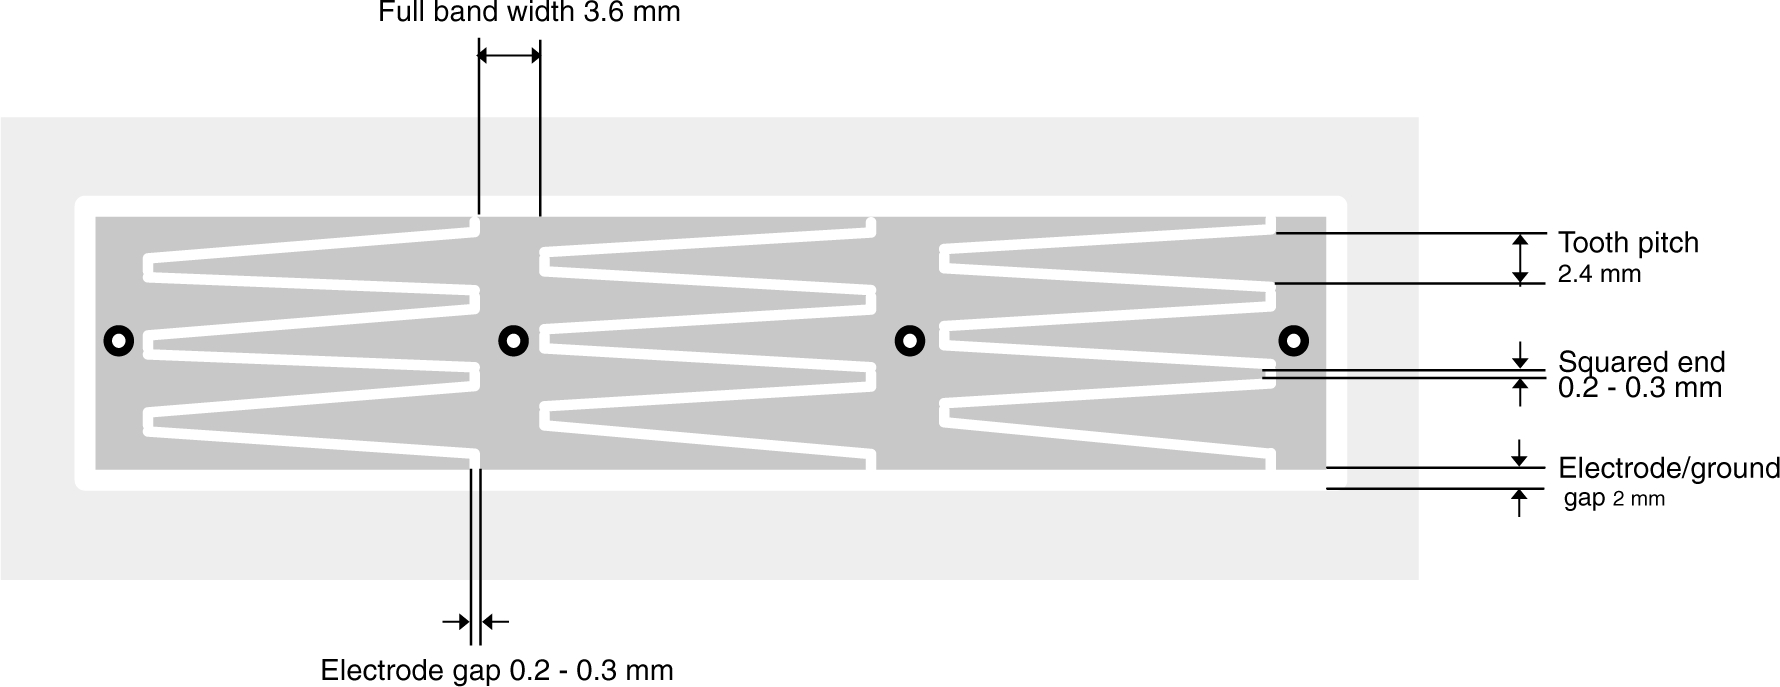
\includegraphics[scale=0.25]{Image/59.jpg} 
\end{center}
\caption{Чересстрочный линейный сенсорный датчик (Interlaced linear sensor)}
\end{figure}

\begin{figure}[H]
\begin{center}
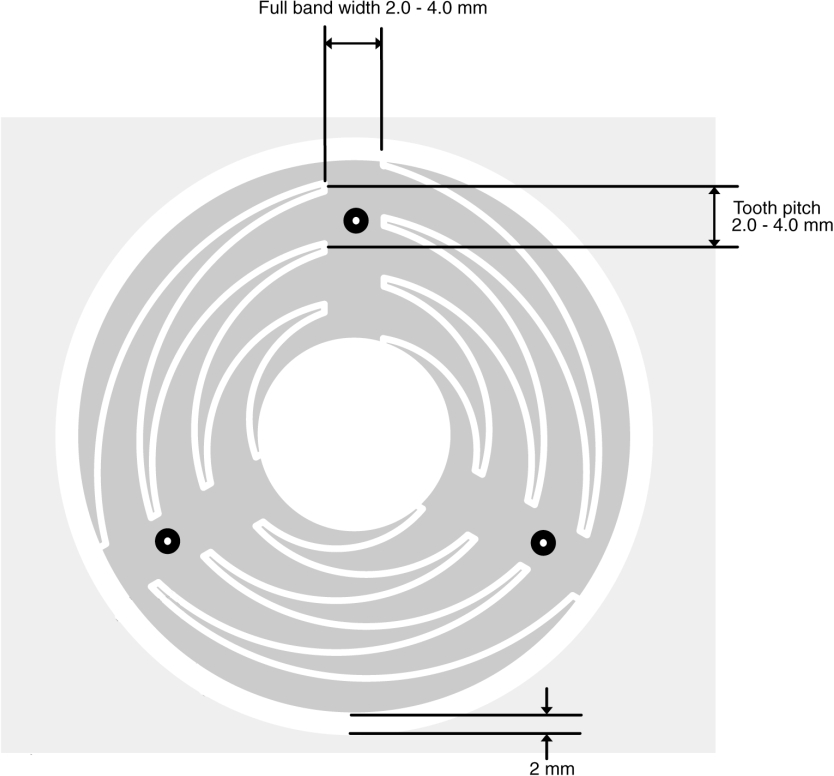
\includegraphics[scale=0.25]{Image/60.jpg} 
\end{center}
\caption{Ротационный сенсорный датчик (Rotary sensor)}
\end{figure}

Многоканальные кнопки подключаются к нескольким группам GPIO и используют несколько каналов, подключенных к измерительным конденсаторам. Интерполяция сигналов между каналами позволяет определять положение касания сенсорной панели. Более подробное описание методов измерения емкости и принципов построения сенсорных панелей приведено в документации \textit{Application note AN2869}.

\section{Библиотека \textit{Touch --  Sensing Library} (TSL)}
\subsection{Описание библиотеки \textit{Touch --  Sensing Library} (TSL)}

Для работы с сенсорными панелями ST Microelectronics разработала библиотеку \textit{Touch --  Sensing Library} --- аналог \textit{Standard Peripherals Library} для работы с периферией. Библиотека позволяет организовывать не только опрос емкостных сенсоров, но и реализуют обработку сигналов с целью снижения влияния внешних помех и повышения стабильности работы. 
	
	 Библиотеки \textit{STM8/STM32 Touch --  Sensing Library} предоставляется в виде открытых исходных кодов на языке С, совместимых со всеми популярными компиляторами (MISRA, Cosmic, IAR, Raisonance C) с примерами использования. Структура библиотек для 8- и 32-битных микроконтроллеров практически идентична -- набор высокоуровневых функций для взаимодействия с прикладными программами, набор вспомогательных сервисов, драйвера устройств, специфичные для каждого из семейств контроллеров, и ядро библиотеки, отвечающее за обработку информации от сенсорных кнопок, калибровку, фильтрацию сигналов, отслеживание изменения окружения. 

Кроме опроса емкостной кнопки в библиотеке предусмотрены алгоритмы обработки сигнала, позволяющие компенсировать негативное влияние таких факторов, как температура, внешнее окружение, изменение напряжения питания. 
 	
 	Ядром библиотеки являются два конечных автомата -- \textit{центральный автомат} (Main State Machine), управляющий последовательностью выполнения действий, и \textit{автомат сенсорной кнопки} (Key State Machine), отслеживающий изменения ее состояния, копия которого запускается для каждой из установленных кнопок.


\begin{figure}[h!]
\begin{center}
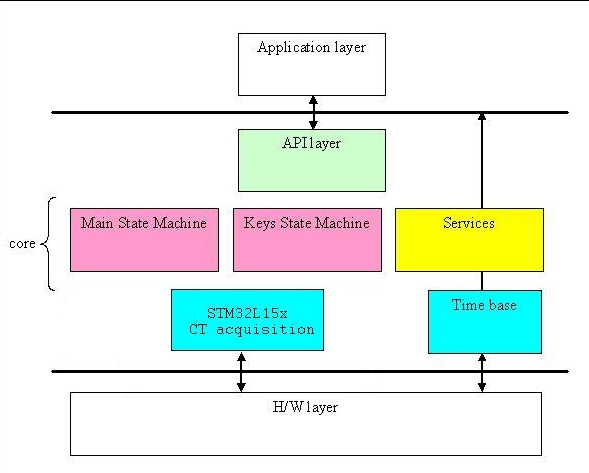
\includegraphics[scale=0.6]{Image/61.jpg} 
\end{center}
\caption{Структура библиотеки \textit{Touch --  Sensing Library}}
\end{figure}

Интерфейс программирования приложений (API, application programming interface) библиотеки доступен через заголовочный файл  \verb\stm32_tsl_api.h\, который содержит описание всех API функций, переменных и структур. Для работы библиотеки используются две функции, которые позволяют инициализировать и запустить центральный автомат:

\verb#TSL_Init()# --- функция вызывается один раз и проводит полную инициализацию системы.

\verb#TSL_Action()# --- функция вызывается периодически в процессе выполнения программы.

Состояния центрального автомата (Main State Machine) хранятся в переменной  \verb\TSLState\ перечисляемого типа \verb\TSLState_T\, определенного в \verb\stm32_tsl_api.h\, а состояния и параметры кнопок хранятся в массиве структур:

\verb#sSCKeyInfo[]# --- для одноканальных кнопок (Single\_Channel\_Complete\_Info\_T type).

\verb#sMCKeyInfo[]# --- для многоканальных кнопок (Tria\_Channel\_Complete\_Info\_T type).

Ядро библиотеки \textit{Touch --  Sensing Library} состоит из следующих файлов:
\begin{itemize}
\item \verb\stm32_tsl_singlechannelkey.c\, \verb\stm32_tsl_singlechannelkey.h\ --- эти файлы содержат функции управления центральным автоматом для одноканальных кнопок и другие функции, выделенные для этого типа кнопок.
\item \verb\stm32_tsl_multichannelkey.c\, \verb\stm32_tsl_multichannelkey.h\ --- эти файлы содержат функции управления центральным автоматом для многоканальных кнопок и другие функции, выделенные для этого типа кнопок, например, вычисление положения нажатия на сенсорную панель.

\item \verb\stm32_tsl_services.c\, \verb\stm32_tsl_services.h\ --- содержат функции, необходимы для кнопок обоих типов.

\item \verb\stm32_tsl_internal.h\ --- файл содержит прототипы функций и макросы для работы TSL
\end{itemize}



\subsection{Центральный автомат}
Центральный автомат (Main State Machine) управляет последовательностью действий, выполняемых системой.  Автомат определен в функции \verb\TSL_Action()\. Элементами перечисляемого типа \verb\TSLState_T\ являются целочисленные константы, отображающие состояния автомата:

\begin{itemize}
\item \verb\TSL_IDLE_STATE\ --- стабильное состояние, в котором все действия завершены. Данное состояние всегда присутствует. Используется для синхронизации TSL с программой.

\item \verb\TSL_SCKEY_P1_ACQ_STATE\ --- перенос заряда от первой группы одноканальных кнопок (first bank acquisition). Данное состояние всегда присутствует.

\item \verb\TSL_SCKEY_P1_PROC_STATE\ --- обработка информации от первой группы одноканальных кнопок (first bank signal processing). Данное состояние всегда присутствует.

\item \verb\TSL_SCKEY_P2_ACQ_STATE\ --- перенос заряда от второй группы одноканальных кнопок (second bank acquisition).

\item \verb\TSL_SCKEY_P2_PROC_STATE\ --- обработка информации от второй группы одноканальных кнопок (second bank signal processing).

\item \verb\TSL_SCKEY_P3_ACQ_STATE\ --- перенос заряда от третьей группы одноканальных кнопок (third bank acquisition).

\item \verb\TSL_SCKEY_P3_PROC_STATE\ ---  обработка информации от третьей группы одноканальных кнопок (third bank signal processing).

\item \verb\TSL_MCKEY1_ACQ_STATE\ --- перенос заряда первой многоканальной кнопки.

\item \verb\TSL_MCKEY2_ACQ_STATE\ --- перенос заряда второй многоканальной кнопки.

\item \verb\TSL_MCKEY_PROC_STATE\ --- обработка сигналов от первой и второй многоканальных кнопок.

\item \verb\TSL_ECS_STATE\ --- Environment Control System process. Это состояние всегда присутствует.
\end{itemize}

Все дополнительные состояние инициализируются в файле \verb\stm32_tsl_conf.h\.
\begin{figure}[h!]
\begin{center}
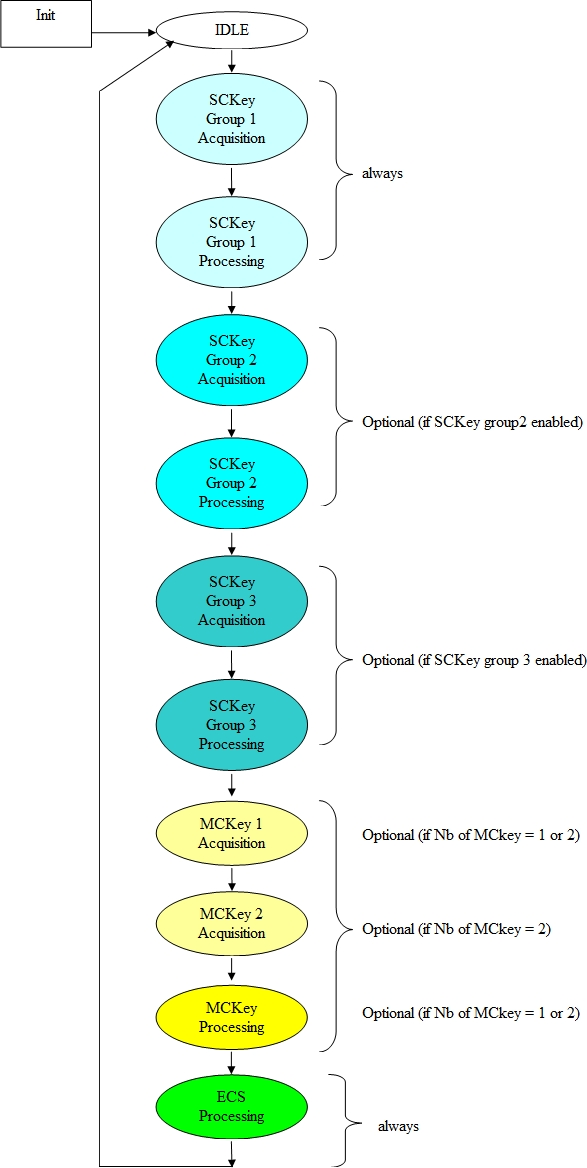
\includegraphics[scale=0.45]{Image/62.jpg} 
\end{center}
\caption{Граф центрального автомата (Main State Machine)}
\end{figure}


\subsection{Фильтры устранения дребезга (Debounce Filters)}

\textit{Debouncing} --- устранение дребезга. Данный фильтр позволяет фиксировать нажатие на сенсорную панель (кнопку) только в случае, если кнопка нажата в течение нескольких циклов работы центрального автомата. Количество циклов определяется пользователем во время настройки фильтра в файле \verb\stm32_tsl_conf.h\. Фильтр помогает устранить эффект дребезга контактов, позволяя фиксировать только истинное нажатие. Фильтр используется при обнаружении нажатия (key detection), обнаружении конца нажатия (key end detection) и до входа в состоянии калибровки (calibration state). Счетчик, отвечающий за количество циклов, устанавливается в состоянии инициализации и уменьшается каждый цикл центрального автомата. Для установки счетчика определены три константы в файле конфигурации \verb\stm32_tsl_conf.h\:
\begin{itemize}
\item \verb\DETECTION_INTEGRATOR_DEFAULT\ --- определяет количество циклов, необходимых для обнаружения нажатия на сенсорную панель.

\item \verb\END_DETECTION_INTEGRATOR_DEFAULT\ --- определяет количество циклов, необходимых для обнаружения конца нажатия.

\item \verb\RECALIBRATION_INTEGRATOR_DEFAULT\ --- определяет количество циклов, необходимых для калибровки.
\end{itemize}
\verb\DETECTION_INTEGRATOR_DEFAULT\ и \verb\END_DETECTION_INTEGRATOR_DEFAULT\ могут принимать значения:
\begin{itemize}
\item \verb\0\ --- фильтр устранения дребезга отключен, обработка информации происходит за первый цикл центрального автомата.
\item \verb\1\ --- два цикла центрального автомата используется для определения нажатия.
\item \verb\2\ --- три цикла центрального автомата используется для определения нажатия.
\item и тд.
\end{itemize}
\begin{figure}[H]
\begin{center}
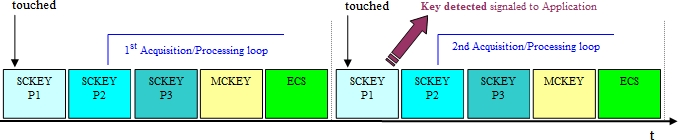
\includegraphics[scale=0.7]{Image/63.jpg} 
\end{center}
\caption{Работа фильтра устранения дребезга в случае использования 2 циклов центрального автомата}
\end{figure}


\subsection{Автомат сенсорной кнопки}

Копия автомата сенсорной кнопки запускается для каждой кнопки. Автомат управляет возможными состояниями кнопки. Автомат определен два раза: в функции \verb\TSL_SCKey_Process()\ для одноканальных кнопок и в функции  \verb\TSL_MCKey_Process()\ для многоканальных кнопок.
Состояния автомата сенсорной кнопки определены в объединении  \verb\KeyState_T\ файле \verb\stm32_tsl_api.h\. Возможны следующие состояния:
\begin{itemize}
\item \verb\IDLE_STATE\ --- кнопка не нажата, ожидание нажатия или калибровки.

\item \verb\PRE_DETECTED_STATE\ --- условие обнаружения нажатия выполнено, запускается счетчик фильтра устранения дребезга.

\item \verb\DETECTED_STATE\ --- кнопка нажата, система ожидает окончания нажатия.

\item \verb\POST_DETECTED_STATE\ --- условие окончания нажатия выполнено, запускается счетчик фильтра устранения дребезга.

\item \verb\PRE_CALIBRATION_STATE\ --- условие калибровки выполнено, запускается счетчик фильтра устранения дребезга.

\item \verb\CALIBRATION_STATE\ --- происходит калибровка сенсорной кнопки. Для этого производится несколько раз перенос заряда для кнопки.

\item \verb\ERROR_STATE\ --- состояние ошибки. Автомат переходит в это состояния при любой появившейся ошибки

\item \verb\DISABLED_STATE\ --- информация от кнопки не обрабатывается. 
\end{itemize}
В процессе инициализации автомат устанавливается в состоянии калибровки (CALIBRATION\_STATE) или, если кнопка отключена программно, в состоянии DISABLED\_STATE.
\begin{figure}[H]
\begin{center}
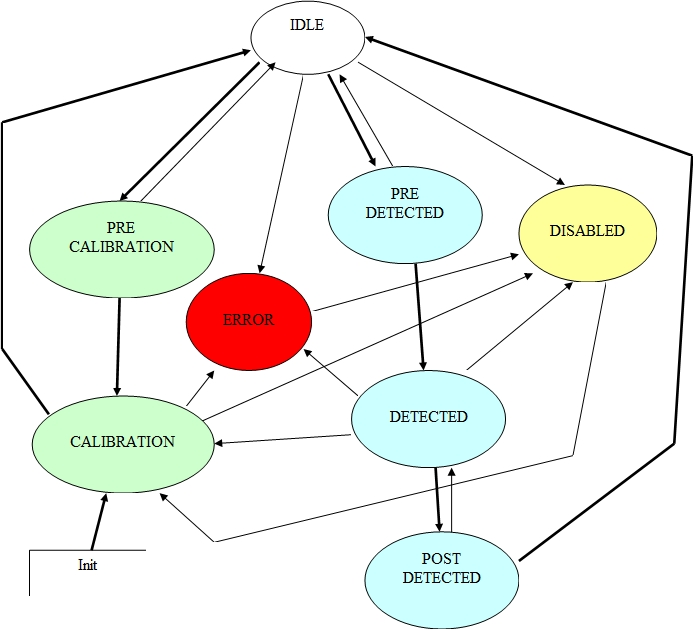
\includegraphics[scale=0.45]{Image/64.jpg} 
\end{center}
\caption{Граф автомата сенсорной кнопки}
\end{figure}




\subsection{Настройка конфигурационного файла библиотеки TSL}

Для настройки \textit{Touch --  Sensing Library} под каждое конкретное приложение используется заголовочный файл \verb\stm32_tsl_conf.h\. Для начала работы с этим файлом необходимо создать копию файла \verb\stm32_tsl_conf_TOADAPT.h\ и переименовать его в \verb\stm32_tsl_conf.h\. 
	
	В начале настройки необходимо выбрать тип используемого микроконтроллера. На отладочной плате STM32L-Discovery установлен микроконтроллер STM32L152RB со 128 Кб Flash. Для этого нужно раскомментировать строчку:
\begin{verbatim}
#define STM32L15XXB_128K (1)  /**< Select this line if the 
                                   STM32L15XXB (128Kb Flash) 
                                   devices are used */
\end{verbatim}
Далее необходимо указать, к какому каналу подключен измерительный конденсатор (Sampling capacitor). Сенсорная панель подключена к 3 группам GPIO (см. UM1079 User manual):
\begin{itemize}
\item PA6, PA7 (group 2)
\item PC4, PC5 (group 9)
\item PB0, PB1 (group 3)
\end{itemize}
Измерительный конденсатор должен быть в каждой группе. В каждой группе находится по 2 канала (см. рисунок \ref{PortInGroup}). Для единообразия измерительный конденсатор подключается ко второму каналу каждой группы:
\begin{verbatim}
#define SAMP_CAP_CH   (CH2)  /**< Possible values are CH1, 
                                  CH2, CH3 and CH4 */
\end{verbatim}
Следующий блок отвечает за настройки одноканальных кнопок в первой группе одноканальных кнопок. Количество кнопок указывается в именованной константе:
\begin{verbatim}
#define SCKEY_P1_KEY_COUNT  (1)
\end{verbatim}
Установить канал для кнопки. Выбранный канал должен быть отличен от канала, на котором находится измерительный конденсатор.
\begin{verbatim}
#define SCKEY_P1_CH         (CH1)
\end{verbatim}
Указать группу для каждой кнопки:
\begin{verbatim}
#define SCKEY_P1_A          (GROUP2)
\end{verbatim}
Настройки для одноканальных кнопок второй и третьей группы производятся аналогично. 

В данной работе используется \textit{чересстрочный линейный сенсорный датчик} --- многоканальная кнопка. Одноканальные кнопки не используются. Блок с настройками для всех групп одноканальных кнопок будет выглядеть следующим образом:
\begin{verbatim}
#define SCKEY_P1_KEY_COUNT  (0)
#define SCKEY_P1_CH   (0) /**< Possible values are CH1, 
                               CH2, CH3 and CH4 */
#define SCKEY_P1_A  (0)
#define SCKEY_P1_B  (0)
#define SCKEY_P1_C  (0)
#define SCKEY_P1_D  (0)
#define SCKEY_P1_E  (0)
#define SCKEY_P1_F  (0)
#define SCKEY_P1_G  (0)
#define SCKEY_P1_H  (0)
#define SCKEY_P1_I  (0)
#define SCKEY_P1_J  (0)
\end{verbatim}
Далее происходит настройка многоканальных кнопок. Необходимо указать количество многоканальных кнопок:
\begin{verbatim}
#define NUMBER_OF_MULTI_CHANNEL_KEYS  (1)  /**< Number of multi 
                                                channel keys 
                                                (value from 0 to 2) */
\end{verbatim}
Затем нужно указать используемые каналы и группы. Второй канал \textit{CH2} каждой группы отведен под измерительный конденсатор, поэтому будут использоваться первые каналы каждой группы:
\begin{verbatim}
#define MCKEY1_A_CH  (CH1)      
#define MCKEY1_A     (GROUP2)   
#define MCKEY1_B_CH  (CH1)      
#define MCKEY1_B     (GROUP9)   
#define MCKEY1_C_CH  (CH1)      
#define MCKEY1_C     (GROUP3)
\end{verbatim}
Указать тип многоканальной кнопки. \verb\1\ -- слайдер, \verb\0\ -- колесо.
\begin{verbatim}
#define MCKEY1_TYPE (1)
\end{verbatim}
В случае использования двух многоканальных кнопок, настройка второй многоканальной кнопки производится аналогичным способом.

Затем указываются пороговые значения для одноканальных кнопок.
\begin{itemize}
\item \verb\SCKEY_DETECTTHRESHOLD_DEFAULT\ --- определяет пороговое значения, выше которого кнопка считается нажатой. Значения может быть установлено в диапазоне от 1 до 127.
\item \verb\SCKEY_ENDDETECTTHRESHOLD_DEFAULT\ --- определяет пороговое значения, ниже которого кнопка считается не нажатой (нажатие не фиксируется). Значения может быть установлено в диапазоне от 1 до 127.
\item \verb\SCKEY_RECALIBRATIONTHRESHOLD_DEFAULT\ --- определяет пороговое значения, ниже которого считается что кнопка находится в состоянии калибровки. Значения может быть установлено в диапазоне от -1 до -128.
\item \verb\SCKEY_MIN_ACQUISITION\ и \verb\SCKEY_MAX_ACQUISITION\ --- определяют минимальное и максимальное значения для переноса заряда на измерительный конденсатор. Если значение вне этого диапазона, кнопка переходит в состоянии ошибки. Значения устанавливаются в диапазоне от 1 до 65535.
\end{itemize}
Пороговые значения для многоканальных кнопок устанавливаются подобно одноканальным и имеют такой же физический смысл:
\begin{verbatim}
#define MCKEY_DETECTTHRESHOLD_DEFAULT          (70)
#define MCKEY_ENDDETECTTHRESHOLD_DEFAULT       (40) 
#define MCKEY_RECALIBRATIONTHRESHOLD_DEFAULT   (-70)
...
#define MCKEY_MIN_ACQUISITION                  (150)
#define MCKEY_MAX_ACQUISITION                  (5000)
\end{verbatim}
Дальнейшие именованные константы файла \verb\stm32_tsl_conf.h\ применяется для более точной настройки библиотеки под конкретное приложение. Процедура настройки и значения всех параметров подробно описаны в файле \verb\stm32_ts_driver_um.chm\ (скомпилированный файл справки в формате HTML), который всегда находится в каталоге библиотеки.

\subsection{Подключение библиотеки \textit{Touch --  Sensing Library} к проекту}
\begin{enumerate}
\item Создать копию файла \verb\stm32_tsl_conf_TOADAPT.h\, переименовать его в \verb\stm32_tsl_conf.h\
\item Настроить файл \verb\stm32_tsl_conf.h\ в соответствии с требованиями
\item Подключить в исходный файл главной программы \verb\main.c\ заголовочный файл \verb\stm32_tsl_api.h\:
\begin{verbatim}
 #include "stm32_tsl_api.h"
\end{verbatim} 

\item Добавить заголовочные и исходные файлы библиотеки в созданный проект.
\item В главной программе вызвать функцию \verb\TSL_Init()\ для инициализации центрального автомата.
\item Инициализировать кнопки, используемые приложением:
\begin{verbatim}
sMCKeyInfo[0].Setting.b.IMPLEMENTED = 1;
sMCKeyInfo[0].Setting.b.ENABLED = 1;
sMCKeyInfo[0].DxSGroup = 0x00; 
\end{verbatim}
\item Вызвать функции \verb\TSL_Action()\ в бесконечном цикле приложения.
\end{enumerate}
Для упрощения работы с состояниями сенсорной панели удобно объявить две именованные константы:
\begin{verbatim}
#define SLIDER_DETECTED (sMCKeyInfo[0].Setting.b.DETECTED)
#define SLIDER_POSITION (sMCKeyInfo[0].UnScaledPosition)
\end{verbatim}
\verb\SLIDER_DETECTED\ отвечает за обнаружение нажатия и \verb\SLIDER_POSITION\ возвращает позицию нажатия (положение точки касания). Все используемые в этом объявлении структуры определены в файле \verb\stm32_tsl_api.h\.

\section{Прерывания}
\subsection{Общие сведения}

Для обработки событий, происходящих по отношению к главной программе асинхронно, лучше всего подходит механизм \textit{прерываний}. \textit{Прерывание} (interrupt) --- сигнал, сообщающий процессору, о наступлении какого-либо события, требующего немедленной реакции, например, нажатие клавиши на клавиатуре. При возникновении прерывания, происходит остановка главной программы, а управление передается \textit{обработчику прерываний} (interrupt handler) или \textit{процедуре обслуживания прерываний} (interrupt service routine (ISR)). После выполнения программы обработчика прерывания, управление передается главной программе, и программа возобновляет свою работу с места остановки.

Каждому прерыванию в соответствии ставиться определенное число -- \textit{номер прерывания}. Для того чтобы связать номер прерывания с адресом обработчика прерывания используется \textit{таблица векторов прерываний}. Элементы таблицы векторов прерываний называются \textit{векторами прерываний}. 

В зависимости от источника возникновения сигнала прерывания делятся на:
\begin{itemize}
\item \textit{Асинхронные или внешние (аппаратные)} --- события, которые исходят от внешних источников (например, периферийных устройств) и могут произойти в любой произвольный момент: сигнал от таймера, сетевой карты или дискового накопителя, нажатие клавиш клавиатуры, движение мыши. Факт возникновения в системе такого прерывания трактуется как \textit{запрос на прерывание} (Interrupt request, IRQ);
\item \textit{Синхронные или внутренние} --- события в самом процессоре как результат нарушения каких-то условий при исполнении машинного кода: деление на ноль или переполнение, обращение к недопустимым адресам или недопустимый код операции;
\item\textit{ Программные (частный случай внутреннего прерывания)} --- инициируются исполнением специальной инструкции в коде программы. Программные прерывания, как правило, используются для обращения к функциям встроенного программного обеспечения (firmware), драйверов и операционной системы.
\end{itemize}

Часто при выполнении критических участков программ, для того чтобы гарантировать выполнение определенной последовательности команд целиком, приходится запрещать прерывания (т.е. сделать систему нечувствительной ко всем или отдельным прерываниям), следовательно в зависимости от возможности запрета внешние прерывания делятся на:
\begin{itemize}
\item \textit{ Маскируемые} --- прерывания, которые можно запрещать установкой соответствующих битов в регистре маскирования прерываний. 
\item \textit{ Немаскируемые} (Non maskable interrupt, NMI) --- обрабатываются всегда, независимо от запретов на другие прерывания. К примеру, такое прерывание может быть вызвано сбоем в микросхеме памяти.
\end{itemize}

Важным свойством прерывания является \textit{приоритет}. Если при обработке прерывания поступает прерывания с более высоким приоритетом, останавливается работа обработчика прерывания, и управление передается обработчику прерывания с более высоким приоритетом. Работа обработчика не может быть остановлена поступлением запроса на прерывание с более низким приоритетом. При одновременном поступлении двух и более запросов на прерывание, прерывания будут обрабатываться в соответствии с приоритетом. При одновременном поступлении двух и более запросов на прерывание с одинаковым приоритетом, прерывания будут обрабатываться в соответствии с возрастанием номера прерывания.
\subsection{Настройка прерываний}

В ядро Cortex-M3 входит \textit{блок контроллера вложенных прерываний по вектору} (Nested vectored interrupt controller, NVIC). Контроллер поддерживает одно немаскируемое прерывание и еще до 240 внешних линий прерывания, которые можно подключить к пользовательским УВВ. В ядре Cortex поддерживается еще 15 дополнительных источников прерываний, использующихся для обработки внутренних исключительных ситуаций ядра Cortex. Контроллер осуществляет:
\begin{itemize}
\item Разрешение и запрет вызова прерываний;
\item Назначение и динамическое изменение приоритета прерываний (16 уровней от 0 (максимального) до 15);
\item Автоматическое сохранение и восстановление контекста данных при обработке одиночных и вложенных прерываний;
\item При одновременном вызове, механизм отложенных прерываний позволяет отложить обработку менее приоритетного прерывания, без возврата в фон и восстановления контекста данных.
\end{itemize}

Определённым событиям, связанным с работой периферийных модулей STM32, назначены отдельные источники прерываний с соответствующими порядковыми номерами. Номера прерываний \textit{IRQn} для микроконтроллеров определённой подгруппы объявлены в разделе \textit{STM32 specific Interrupt Numbers} заголовочного файла \verb\stm32l1xx.h\ в CMSIS:
\begin{verbatim}
typedef enum IRQn
{
...
RCC_IRQn     = 5,      /*!< RCC global Interrupt */
EXTI0_IRQn   = 6,      /*!< EXTI Line0 Interrupt */
EXTI1_IRQn   = 7,      /*!< EXTI Line1 Interrupt */
EXTI2_IRQn   = 8,      /*!< EXTI Line2 Interrupt */
EXTI3_IRQn   = 9,      /*!< EXTI Line3 Interrupt */
EXTI4_IRQn   = 10,     /*!< EXTI Line4 Interrupt */
...
} IRQn_Type;
\end{verbatim}
Для разрешения прерываний от определенного источника используется функция, объявленная в заголовочном файла \verb\core_cm3.h\\footnote{Не забудьте, что IAR, начиная с версии 6.2, использует собственные файлы}
\verb\core_cm3.h\, \verb\core_cm3.c\. библиотеки CMSIS:
\begin{verbatim}
void NVIC_EnableIRQ(IRQn_Type IRQn)
\end{verbatim}
Для изменения приоритета прерывания используется функция, объявленная в заголовочном файла \verb\core_cm3.h\:  
\begin{verbatim}
void NVIC_SetPriority(IRQn_Type IRQn, uint32_t priority)
\end{verbatim}
Например, для установки самого низкого приоритета для внешнего прерывания, поступающего по линии 0, используется команда:
\begin{verbatim}
NVIC_SetPriority (EXTI0_IRQn, 15);
\end{verbatim}

Для работы с внешними прерываниями в микроконтроллере существует \textit{контроллер внешних прерываний (событий)} (External interrupt/event controller, EXTI). Контроллер позволяет генерировать прерывания в зависимости от состояния пина соответствующего порта.
\begin{figure}[h]
\begin{center}
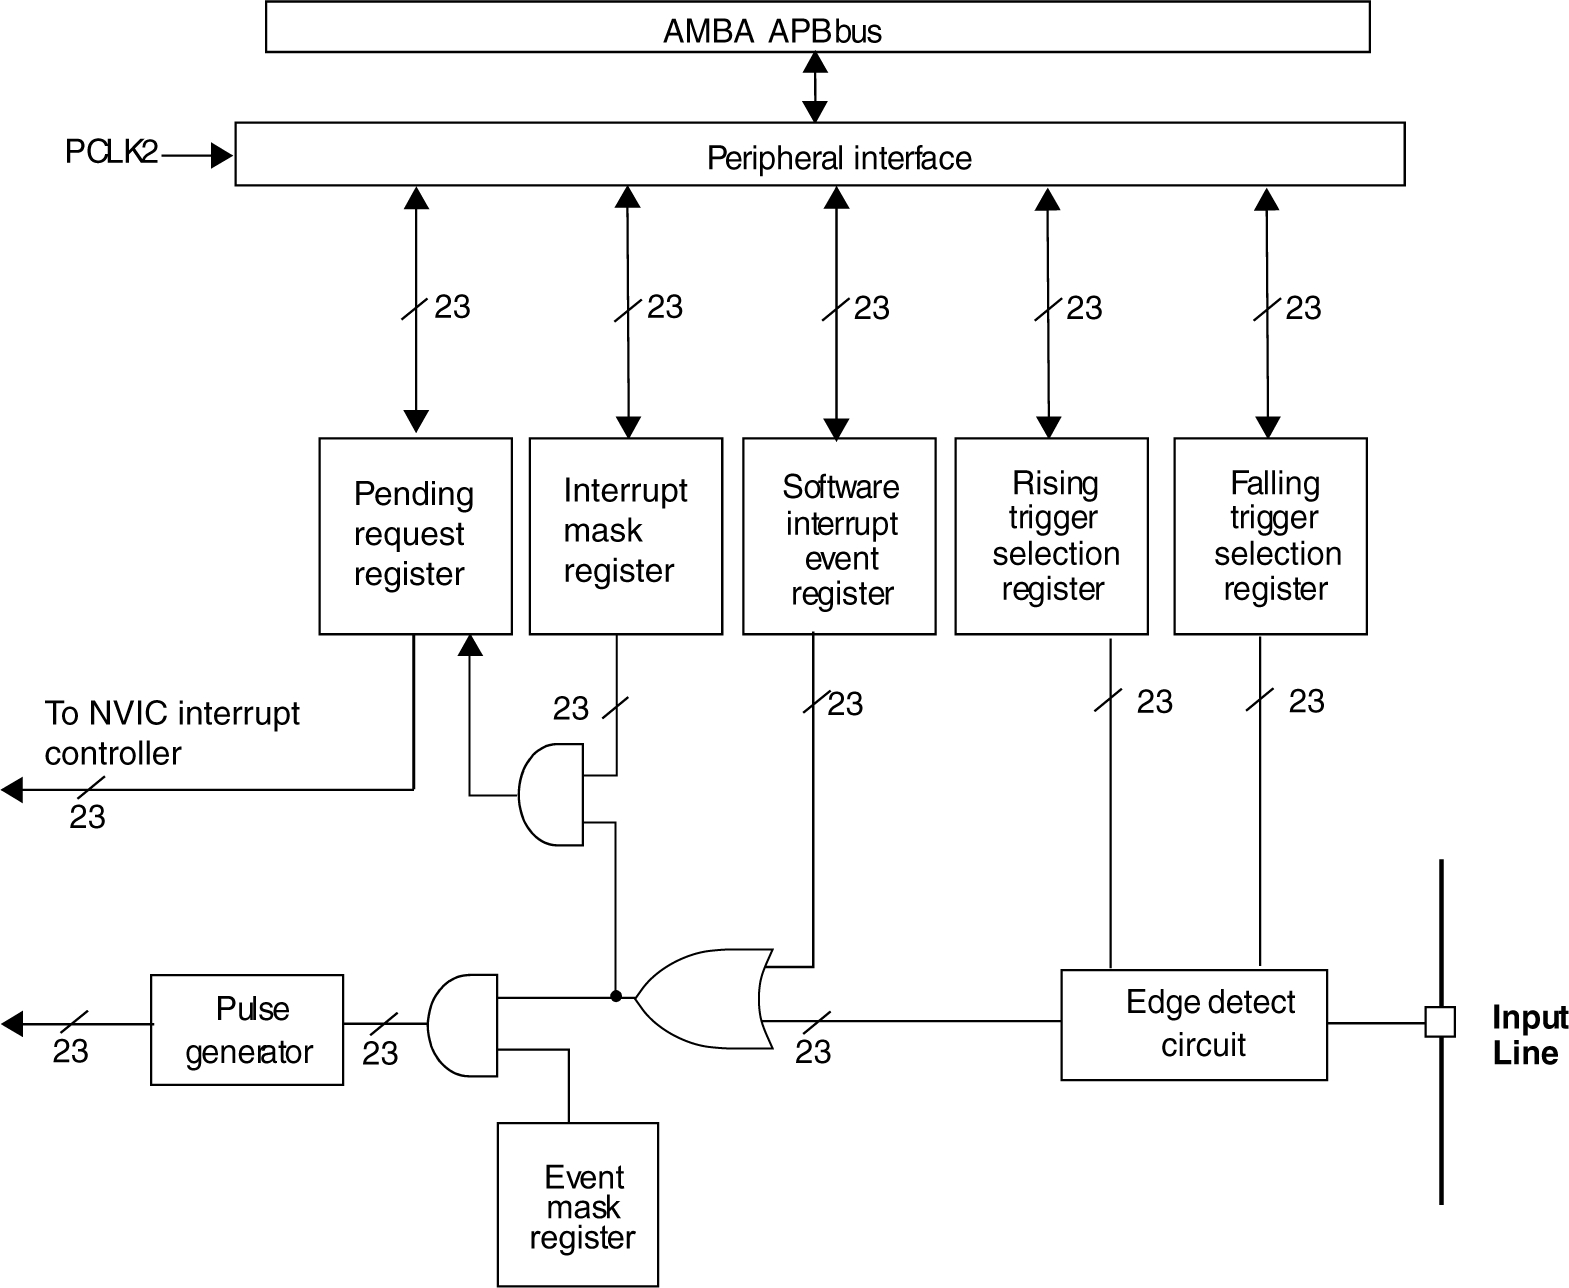
\includegraphics[scale=0.15]{Image/65.jpg} 
\end{center}
\caption{Схема контроллера внешних прерываний}
\end{figure}
Подключение линий ввода - вывода производится посредством 16 мультиплексоров, по одному семивходовому мультиплексору на одну линию прерывания. При возникновении условий для пинов 0 -- 4 генерируется запрос на прерывание по раздельным линиям прерывания \textit{EXTI0\_IRQn -- EXTI4\_IRQn}, для выводов 5 -- 9 и 10 -- 15 по групповым линиям \textit{EXTI9\_5\_IRQn} и \textit{EXTI15\_10\_IRQn} соответственно. Прерывание можно настроить только для пинов, настройка прерываний на порты не производится.

\begin{figure}[H]
\begin{center}
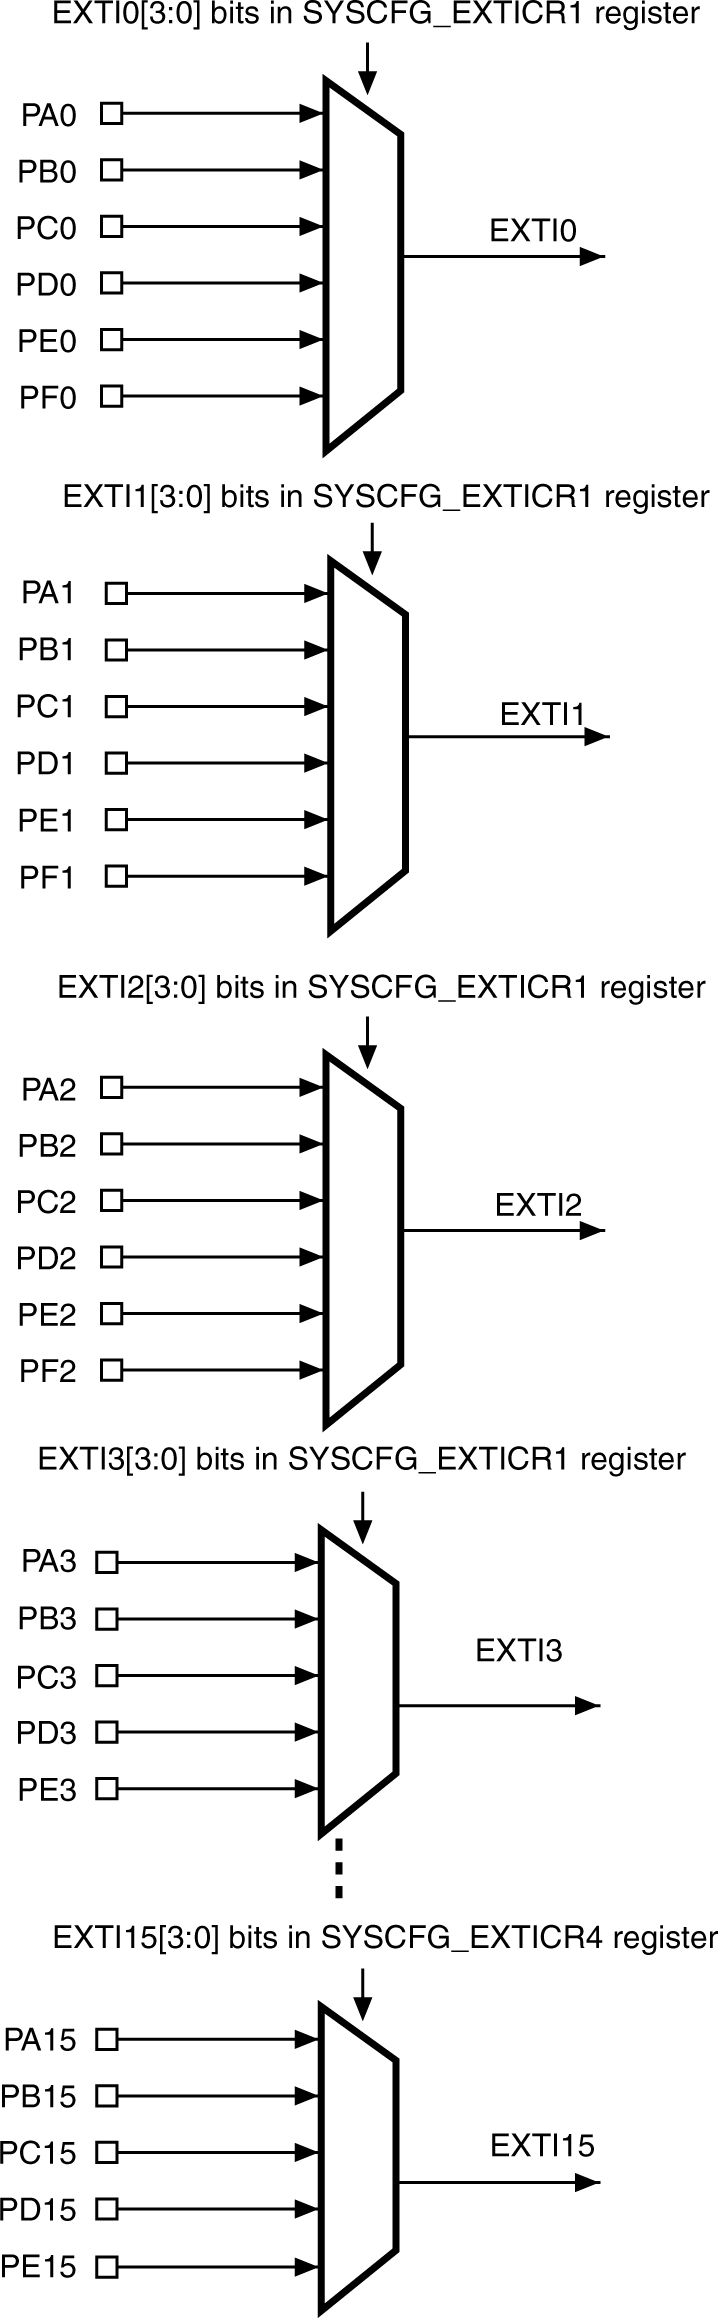
\includegraphics[scale=0.18]{Image/66.jpg} 
\end{center}
\caption{Схема подключения линий ввода-вывода}\label{InputOutput}
\end{figure}

Для генерирования внешнего прерывания необходимо настроить и разрешить соответствующую линию прерывания. Настройка производится указанием по фронту или по срезу сигнала пина формировать прерывание. Разрешение прерывания происходит установкой \verb\1\ в соответствующий бит регистра маскирования \textit{EXTI\_IMR} (EXTI interrupt mask register) для формирования немаскируемого прерывания. В процессе обработки прерывания в регистре ожидания \textit{EXTI\_PR} (EXTI pending register) записью единицы необходимо сбросить бит (флаг) события вызвавшего данное прерывание.
	
Пользовательская кнопка \textit{User} на отладочной плате STM32L-Discovery подключена к порту PA0, соответственно необходимо разрешить линию прерывания \textit{EXTI0} (см. рисунок \ref{InputOutput}).

\begin{figure}[H]
\begin{center}
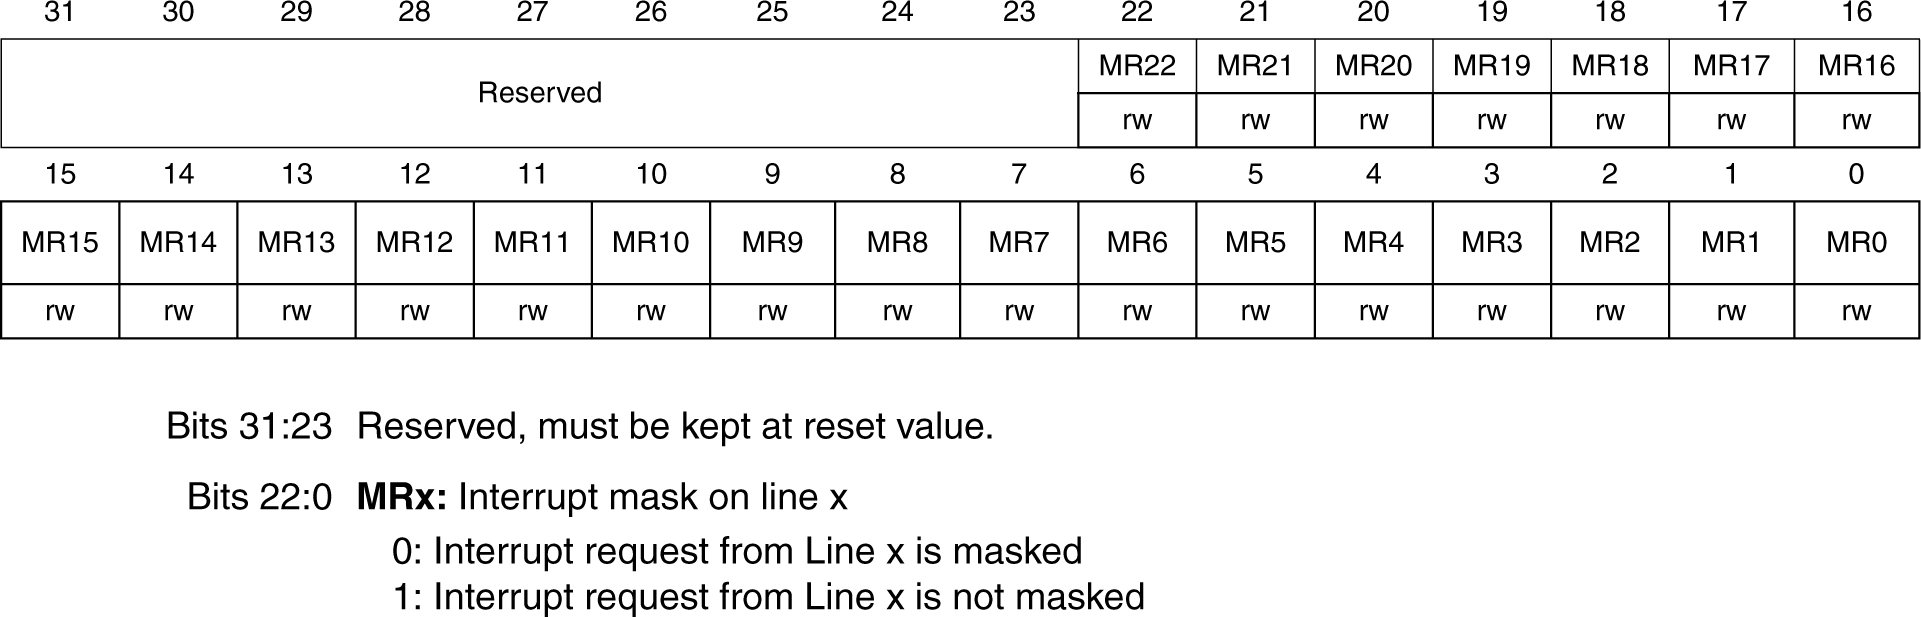
\includegraphics[scale=0.25]{Image/67.jpg} 
\end{center}
\caption{Регистр \textit{EXTI\_IMR} (EXTI interrupt mask register)}
\end{figure}
Для разрешение линии прерывания \textit{EXTI0} необходимо в регистр маскирования \textit{EXTI\_IMR} (EXTI interrupt mask register) установить \verb\1\ в 0 разряд \cite{inter}
\begin{verbatim}
EXTI->IMR |= EXTI_IMR_MR0; 
// EXTI->IMR |= 0x1;
\end{verbatim}
Для настройки прерывания по фронту сигнала используется регистр \textit{EXTI\_RTSR} (EXTI Rising edge trigger selection register), по срезу сигнала регистр \textit{EXTI\_FTSR} (EXTI Falling edge trigger selection register).
\begin{figure}[H]
\begin{center}
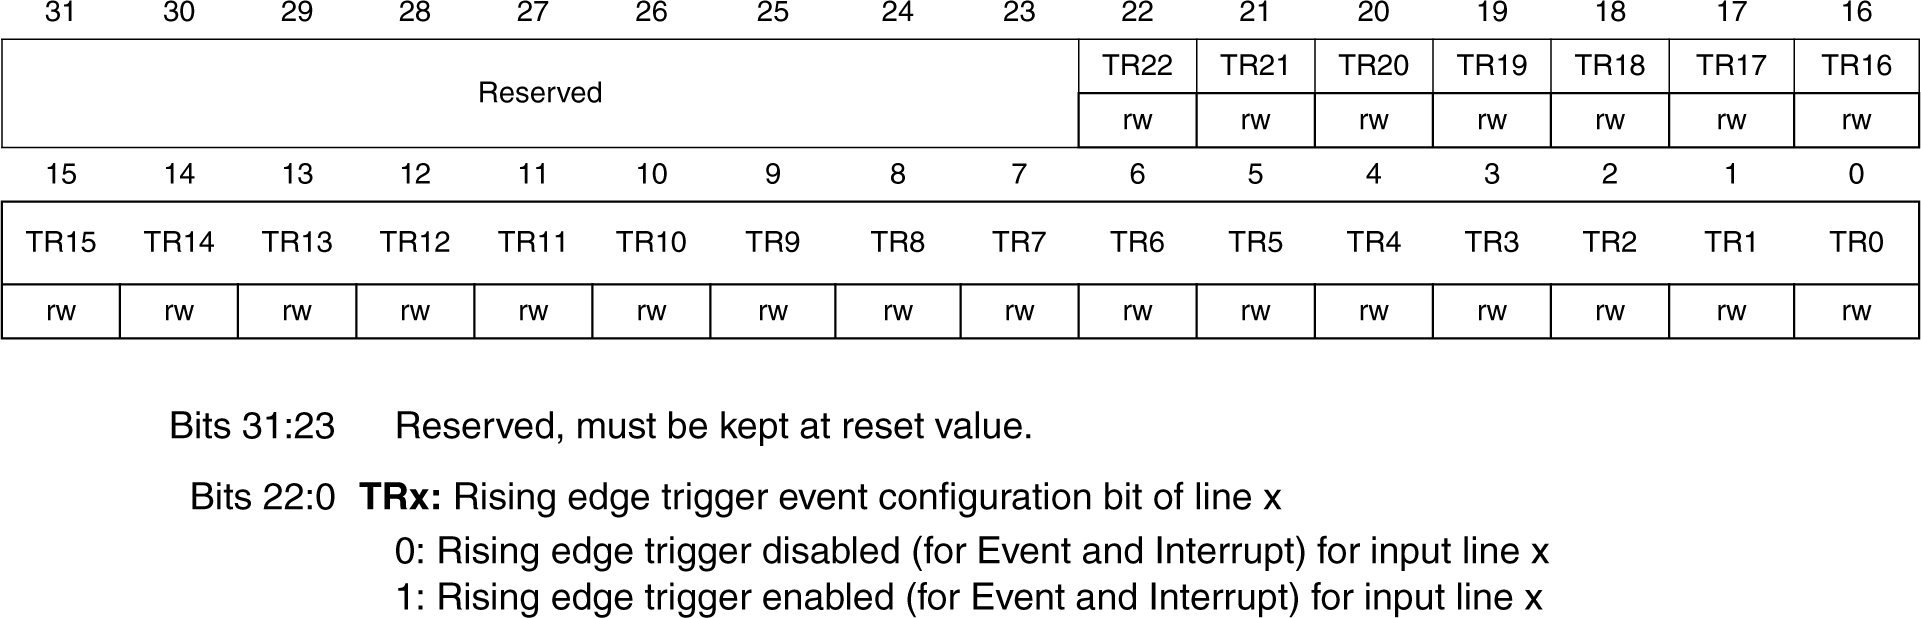
\includegraphics[scale=0.25]{Image/68.jpg} 
\end{center}
\caption{Регистр \textit{EXTI\_RTSR} (EXTI Rising edge trigger selection register)}
\end{figure}
\begin{figure}[H]
\begin{center}
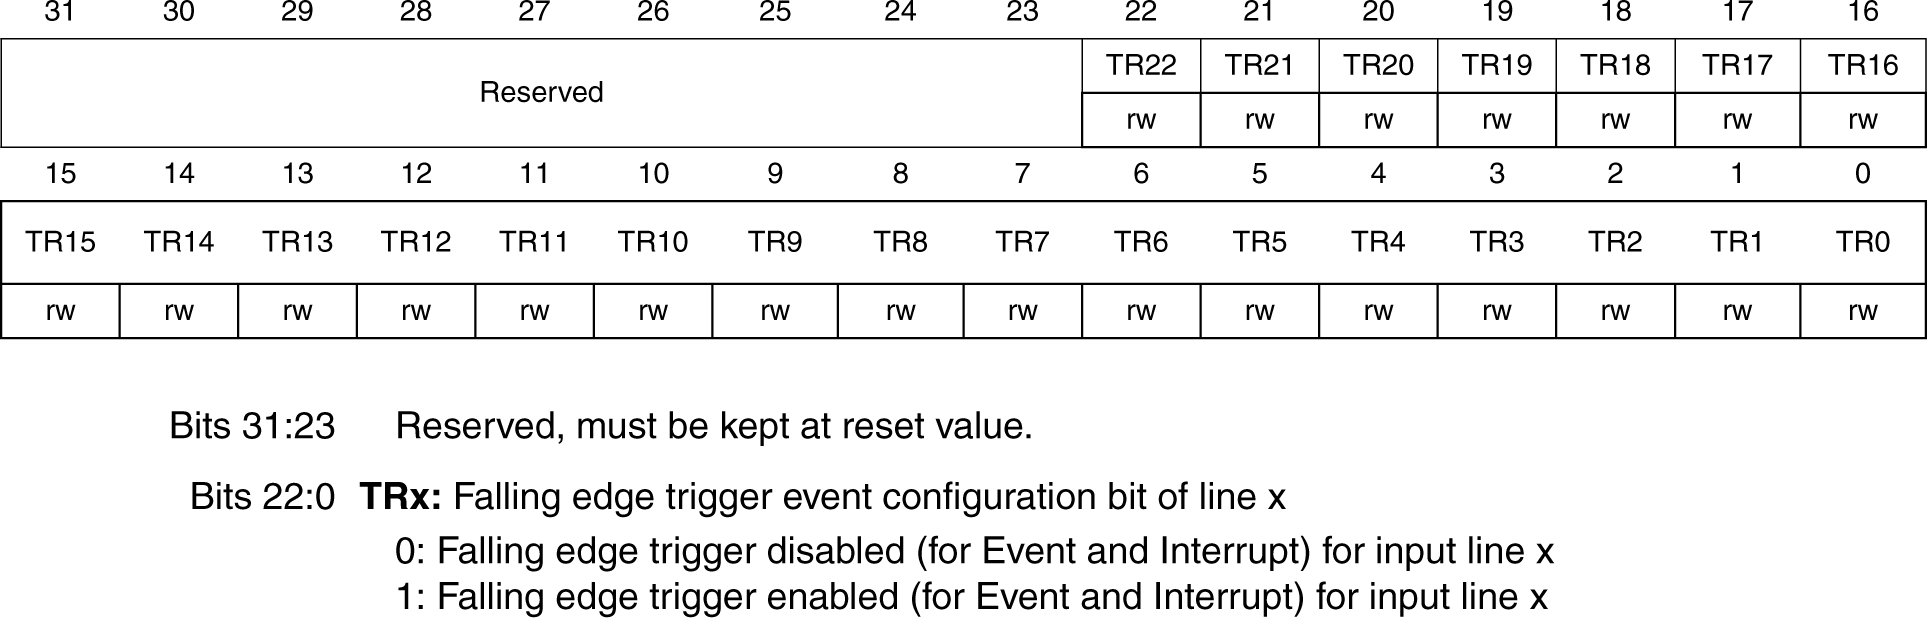
\includegraphics[scale=0.25]{Image/69.jpg} 
\end{center}
\caption{Регистр \textit{EXTI\_FTSR} (EXTI Falling edge trigger selection register)}
\end{figure}
Для настройки прерываний по фронту и срезу для линии прерывания \textit{EXTI0} необходимо установить 1 в 0 разряд обоих регистров:
\begin{verbatim}
EXTI->RTSR |= EXTI_RTSR_TR0;
EXTI->FTSR |= EXTI_FTSR_TR0;
// EXTI->RTSR |= 0x1; 
// EXTI->FTSR |= 0x1;
\end{verbatim}

Регистр \textit{EXTI\_SWIER} (EXTI software interrupt event register) используется для программного генерирования прерываний. Для сброса бита события вызвавшего прерывание используется регистр ожидания \textit{EXTI\_PR} (EXTI pending register). Для сброса прерывания произошедшего по линии прерывания \textit{EXTI0} нужно установить \verb\1\ в 0 разряд:
\begin{verbatim}
EXTI->PR |= EXTI_PR_PR0;
// EXTI->PR |= 0x1;
\end{verbatim}
\begin{figure}[H]
\begin{center}
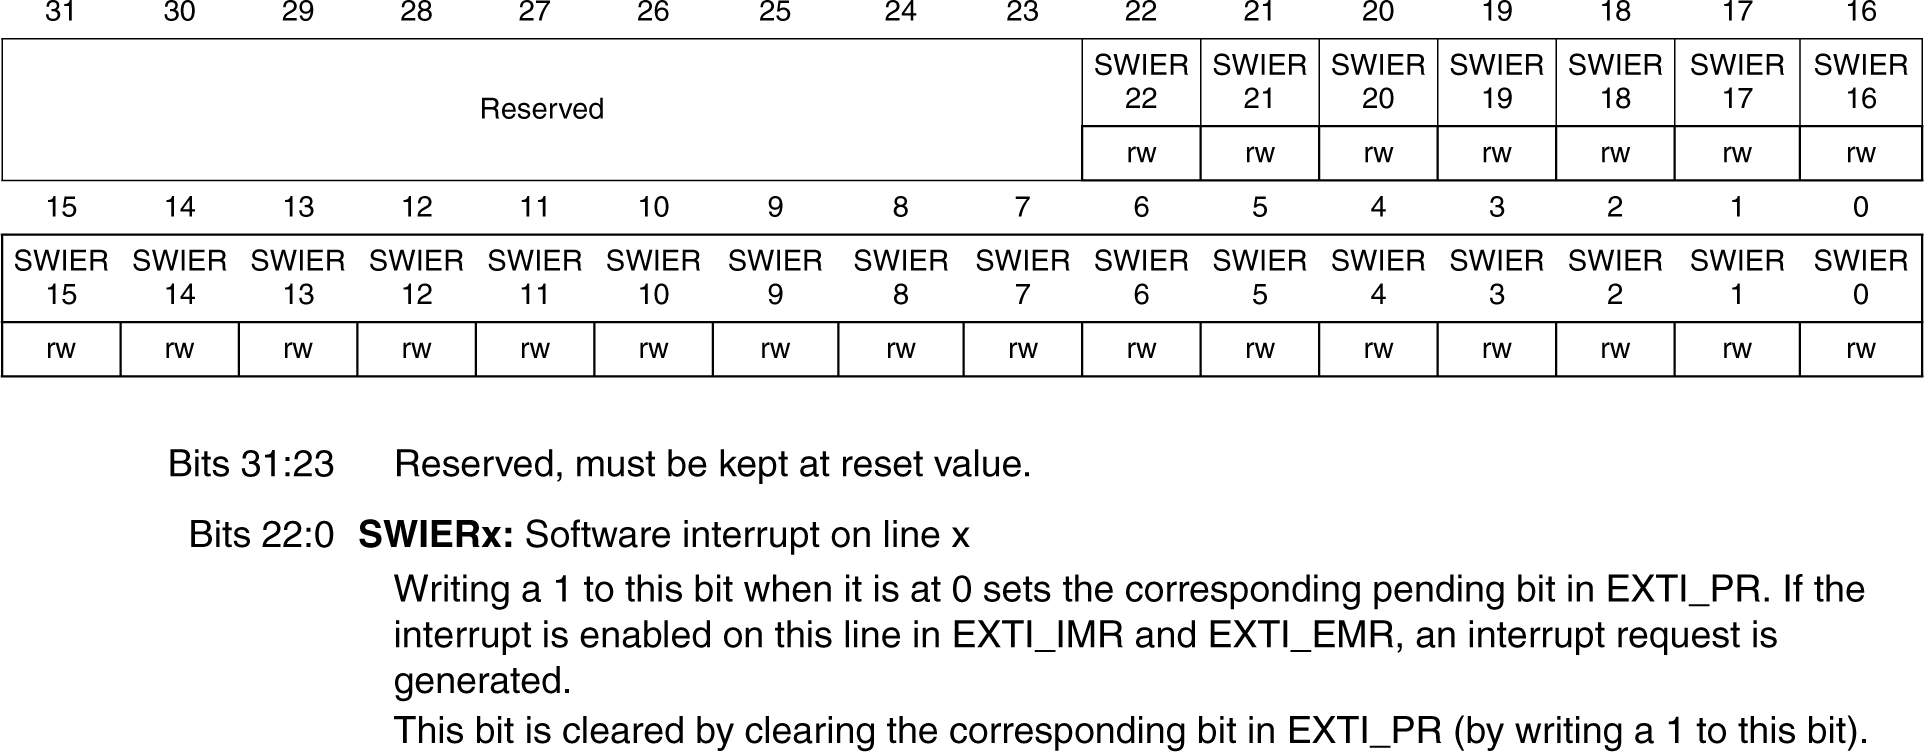
\includegraphics[scale=0.25]{Image/70.jpg} 
\end{center}
\caption{Регистр \textit{EXTI\_SWIER} (EXTI software interrupt event register)}
\end{figure}
\begin{figure}[H]
\begin{center}
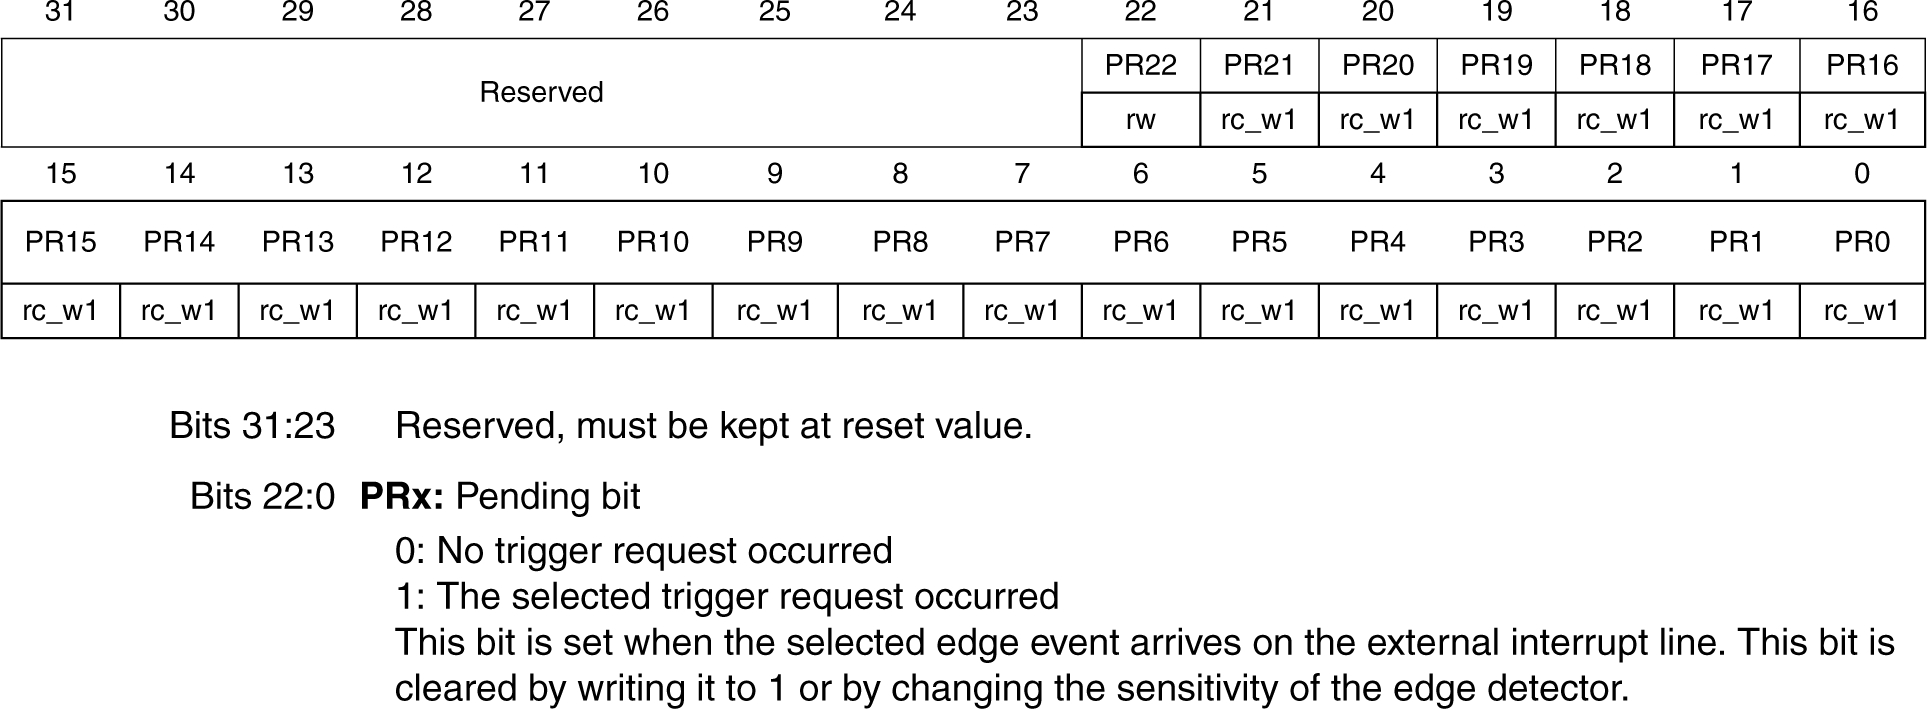
\includegraphics[scale=0.25]{Image/71.jpg} 
\end{center}
\caption{Регистр \textit{EXTI\_PR} (EXTI pending register)}
\end{figure}

Обработчик прерывания имеет следующий вид:
\begin{verbatim}
void ИмяHandler(void)
{
}
\end{verbatim}
где \textit{имя} --- источник прерывания определенный в  \textit{STM32 specific Interrupt Numbers} заголовочного файла  \verb\stm32l1xx.h\ без суффикса  \textit{n}. Для источника  \textit{EXTI0\_IRQn} обработчик прерывания будет иметь вид:
\begin{verbatim}
void EXTI0_IRQHandler(void)
{
}
\end{verbatim}
Все обработчики прерываний, как правило, помещаются в отдельный файл \verb\stm32l1xx_it.c\. Для работы сенсорной панели обязательно наличие обработчика прерываний таймера \textit{SysTick} \cite{systic}. В данной работе никаких действий данного обработчика не требуется, поэтому тело функции остается пустым:
\begin{verbatim}
void SysTick_Handler(void)
{
}
\end{verbatim}

В случае использование прерываний, к проекту должен быть подключен файл \verb\startup_stm32l1xx_md.s\, находящийся в папке \verb#CMSIS/DeviceSupport/ST/STM32L1xx/startup/iar#. Данный файл является программой на языке ассемблера, которая содержит в себе самую низкоуровневую инициализацию контроллера. В нем содержится таблица векторов прерываний, инициализация стека, вызов функции \verb\SystemInit()\ из библиотеки CMSIS и последующий вызов функции \verb\main()\.

\section{Библиотечные функции при работе с сенсорной панелью}

В качестве примера работы с отладочной платой ST Microelectronics поставляет файлы \verb\discover_functions.c\, \verb\discover_functions.h\, которые содержат необходимые функции по работе с сенсорной панелью. Функция
\begin{verbatim}
void Slider_value(void);
\end{verbatim}
позволяет работать с сенсорной панелью в режиме слайдера и выводит на экран ЖКИ информацию о точке касания сенсорной панели в процентах.
\begin{figure}[H]
\begin{center}
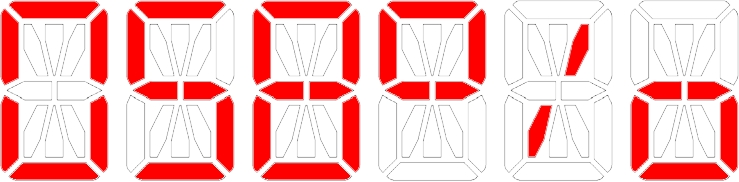
\includegraphics[scale=0.25]{Image/72.jpg} 
\end{center}
\caption{Положение точки касания в процентах на ЖКИ}
\end{figure}


\begin{verbatim}
void Button_value(void);
\end{verbatim}
Функция позволяется рассматривать сенсорную панель как 4 отдельные сенсорные кнопки. При этом на ЖКИ выводится информация о нажатой кнопке. При нажатии на вторую сенсорную кнопку на ЖКИ появиться информация \verb\0*00\.

\begin{figure}[H]
\begin{center}
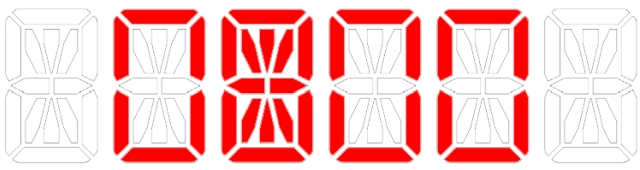
\includegraphics[scale=0.3]{Image/73.jpg} 
\end{center}
\caption{Положение точки касания на ЖКИ}
\end{figure}

\section{Тактирование при работе с сенсорной панелью}
Для работы сенсорной панели необходимо в качестве источника тактового сигнала выбрать \textit{внутренний ВЧ генератор} (HSI). Для включение ВЧ генератора в регистр \textit{RCC\_CR} (Clock control register) необходимо установить \verb\1\ в 0 разряд:
\begin{verbatim}
RCC->CR |= RCC_CR_HSION;
// RCC->CR |= 0x1;
\end{verbatim}
Для стабилизации работы внутреннего ВЧ генератора необходимо некоторое время. Готовность проверяется установкой бита \verb\HSIRDY\ в регистр \textit{RCC\_CR} (Clock control register):
\begin{verbatim}
while(!(RCC->CR & RCC_CR_HSIRDY));
\end{verbatim}

\begin{figure}[H]
\begin{center}
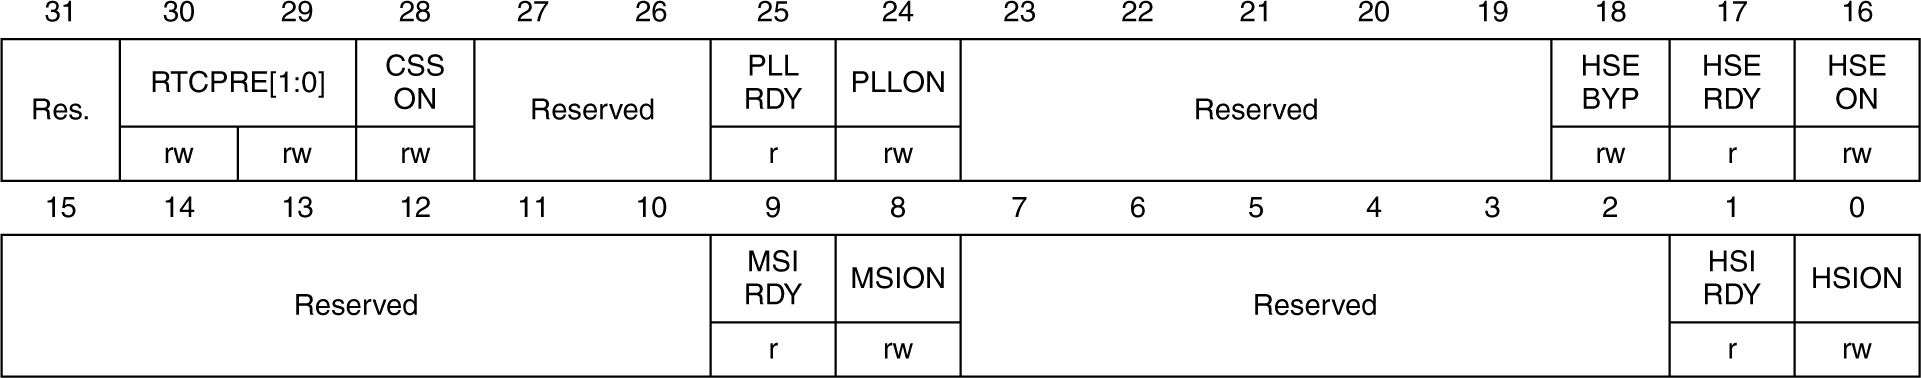
\includegraphics[scale=0.25]{Image/74.jpg} 
\end{center}
\caption{Регистр \textit{RCC\_CR} (Clock control register) }
\end{figure}
Выбор внутреннего ВЧ генератора в качестве источника тактового сигнала происходит установкой \verb\1\ в 0 разряд регистра \textit{RCC\_CFGR} (Clock configuration register):
\begin{verbatim}
RCC->CFGR |= RCC_CFGR_SW_0; 
// RCC->CFGR |= 0x1; 
\end{verbatim}

\begin{figure}[H]
\begin{center}
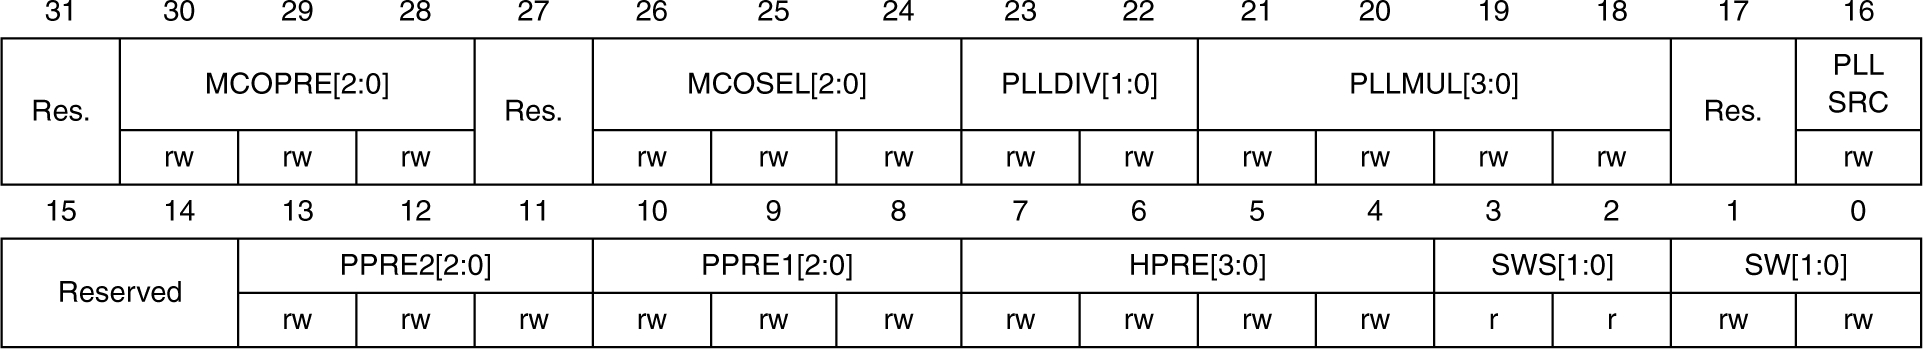
\includegraphics[scale=0.25]{Image/75.jpg} 
\end{center}
\caption{Регистр \textit{RCC\_CFGR} (Clock configuration register)}
\end{figure}
Для сравнения напряжения на измерительном конденсаторе с пороговым уровнем используется \textit{компаратор}. Для тактирования компаратор использует шину \textit{APB1}. Для разрешения тактирование компаратора нужно установить \verb\1\ в 31 разряд регистра \textit{RCC\_APB1ENR} (APB1 peripheral clock enable register):
\begin{verbatim}
RCC->APB1ENR |= RCC_APB1ENR_COMPEN;
// RCC->APB1ENR |= 0x80000000;
\end{verbatim}

\begin{figure}[H]
\begin{center}
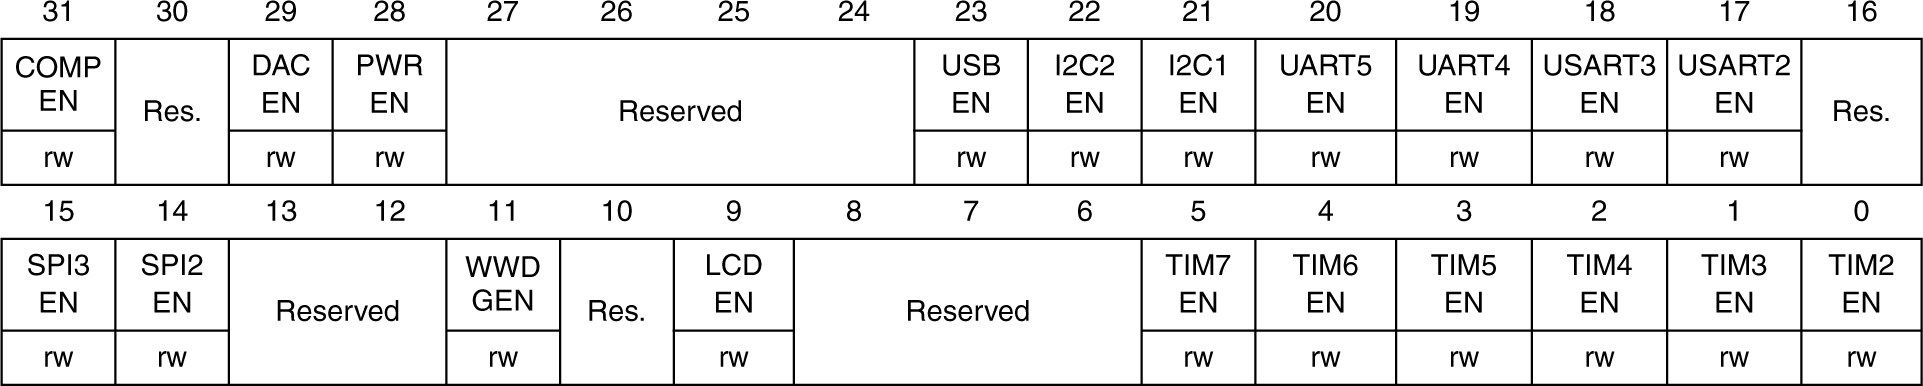
\includegraphics[scale=0.25]{Image/76.jpg} 
\end{center}
\caption{Регистр \textit{RCC\_APB1ENR} (APB1 peripheral clock enable register)}
\end{figure}